\chapter{Theoretical Foundations} \label{chapter:theory}

In this chapter we provide the reader with the minimum conceptual background and theoretical building blocks necessary  to understand this thesis work. We begin our discussion with a general overview of classical and quantum information processing with a Turing machine, followed by an introduction to superconducting quantum circuits. We summarize the method to quantize electrical circuits and apply it to Cooper pair box devices, and in particular to the Transmon that will be used to implement the qubit register of our quantum processor. We then present coplanar waveguide resonators, and introduce circuit quantum electrodynamics on the example of a transmon coupled to a such a resonator. Finally, we consider the case of a nonlinear resonator used as a Josephson bifurcation amplifier since we use such a readout device in our processor architecture.

\section{Classical \& Quantum Information Processing}

\begin{SCfigure}
	\includegraphics[width=8cm]{"./material/figures/introduction/bloch_sphere"}
	\caption{The Bloch sphere representation of a qubit state $\ket{\psi} = \cos{\frac{\theta}{2}}\ket{0}+e^{i\phi}\sin{\frac{\theta}{2}}\ket{1}$. The state $\ket{\psi}$ is fully characterized by specifying its ``latitude'' and ``azimuth'' angles $\theta$ and $\phi$. Pure quantum states will always lie on the surface of the Bloch sphere, whereas mixed quantum states can also lie anywhere inside the sphere.}
	\label{fig:BlochSphere}
\end{SCfigure}

By definition, computing designates the activity of using computer hardware and software to process information, or {\it data}. Classical information processing can be divided in so-called {\it analog and digital information processing}, the former being based on continuously changeable physical quantities whereas the latter is based on incrementally changeable quantities. The fundamental unit of digital information processing is the so-called {\it bit}, which represents a Boolean (true/false) information. The discipline of theoretical computer science has been created to investigate the fundamental limits and properties of classical information processing. One of the main foundational theorems of theoretical computer science is the so-called {\it Church-Turing thesis} which provides a universal computing model by saying (basically) that everything which is computable can be efficiently computed using a {\it Turing machine}. Such a Turing machine, in turn, is a simple theoretical device which is able to run programs that operate on a discrete set of data using a well-specified set of operations. The Turing machine is universal in the sense that any other classical computing device can be efficiently emulated using a Turing machine with the appropriate program and data.

\smallskip

In the early 1980s, Richard Feynman discovered that a classical Turing machine as described above would be unable to efficiently simulate a quantum-mechanical system \citep{feynman_simulating_1982}. He introduced the concept of a {\it quantum Turing machine} that would be able to simulate quantum-mechanical systems in an efficient manner. A few years later, David Deutsch took up Feynman's idea and developed an information processing framework based on quantum mechanics \citep{deutsch_quantum_1985}, coining the terms {\it quantum computing} and {\it quantum information processing}. He showed that by making use of different properties of quantum mechanics, namely, the superposition principle and entanglement, one could solve certain mathematical problems faster than possible with any classical computer \citep{deutsch_quantum_1985}. The work by Deutsch created a large interest in the physics community and led to a huge theoretical and experimental effort aimed at realizing an operational quantum computer and developing quantum algorithms for relevant real-world problems.

\section{Principles of "Conventional" Quantum Computing}

The first scheme imagined for quantum information processing is directly inspired from the classical digital Turing machine: information is stored in a set of quantum two level systems, the {\it quantum bits} or {\it qubits}, forming a quantum register, which is manipulated by sequentially applying unitary (and possibly non-unitary) operators to subsets of qubits in the register, typically one or two. As for a classical Turing machine, any arbitrary operation of this quantum processor can be decomposed as a sequence of gate operations chosen from a surprisingly small set of gates, said universal. The power of such a machine comes from the gates operating on superposed states, which provides an intrinsic parallelism in the processing.
\smallskip
This {\it quantum gate} approach is the method relevant to the present thesis work, and we ignore other approaches introduced more recently such as {\it one-way quantum computing} \citep{raussendorf_one-way_2001}, {\it adiabatic quantum computing} \citep{farhi_quantum_2000} or {\it topological quantum computing} \citep{kitaev_fault-tolerant_2003}. In this section we introduce very briefly quantum bits and quantum gates, as well as some examples of quantum algorithms that are relevant to this work.


\subsection{Quantum Bits and registers}

As in classical computing, one can define in quantum computing a fundamental unit of information: the qubit. Such a qubit is a quantum-mechanical two-level system that can be put in any superposition
%
\begin{equation}
\ket{\psi} = \cos{\frac{\theta}{2}}\ket{0}+e^{i\phi}\sin{\frac{\theta}{2}}\ket{1}
\end{equation}
%
of its two states $\ket{0}$ and $\ket{1}$.
As can be seen, any state can be described by a pair of real numbers $\theta$ and $\phi$ that characterize the amplitude of each of the two basis states and the phase between them. A useful and intuitive representation of such a single-qubit state is the so-called {\it Bloch sphere representation}, shown in fig. \ref{fig:BlochSphere}. The north and south poles of this sphere correspond by convention to the qubit states $\ket{0}$ and $\ket{1}$ (or vice versa). In this representation, any pure state $\ket{\psi}$ is located on a unit sphere. All states lying on the sphere between those two correspond to pure superposition states, which are characterized by their ``latitude'' and ``azimuth'' angles $\theta$ and $\phi$. 

\smallskip

\smallskip

Often it is necessary to describe the qubit not as being in one well-defined pure state but rather being in one of several such states $\ket{\psi_i}$, where for each one of them we can give a classical probability $p_i$ for finding the qubit in that given state. In this case, we can describe the qubit by a {\it so-called}\comment{sorry, Daniel :)} density matrix $\rho = \sum\limits_i p_i \rho_i$, where $\rho_i=\ket{\psi_{i}}\bra{\psi_{i}}$ is the density matrix of the pure state $\ket{\psi_i}$. All single-qubit density matrices $\rho$ are Hermitian $2\times 2$ matrices with non-negative eigenvalues and can thus be written as
%
\begin{equation}
\rho = \left( \begin{array}{cc} \rho_{00} & \rho_{01} \\ \rho_{01}^* & \rho_{11} \end{array} \right),
\end{equation}
%
in the ${\ket{0},\ket{1}}$ basis, with $\rho_{00}$ and $\rho_{11}$ being real numbers and $\rho_{01}$ a complex number. For any state, the matrix has a unity trace $\mathrm{Tr}(\rho)=1$, for pure states we have $\rho=\rho^2$ in addition. The expectation values $\langle A \rangle$ of any operator $A$ acting on the density matrix $\rho$ is given as $\mathrm{Tr}(\rho A)$.

\smallskip

A mixed single-qubit state $\rho$ can also be represented on the Bloch sphere. For this, we decompose $\rho = c_i\sigma_I+c_x\sigma_x+c_y\sigma_y+c_z\sigma_z$, where $c_{i,x,y,z}$ are real coefficients and the identity matrix $\sigma_I$ and Pauli matrices $\sigma_x,\sigma_y,\sigma_z$ are
%
\begin{align}
  \sigma_I  =  \left( \begin{array}{cc} 1 & 0 \\ 0 & 1 \end{array} \right)
 & &  \sigma_x  =  \left( \begin{array}{cc} 0 & 1 \\ 1 & 0 \end{array} \right)
  & & \sigma_y  =  \left( \begin{array}{cc} 0 & -i \\ i  &  0\end{array} \right)
  & & \sigma_z  =  \left( \begin{array}{cc} 1 & 0 \\ 0 & -1 \end{array} \right).
\label{eq:pauli_operators}
\end{align}
% 
We can then plot the vector $(c_x,c_y,c_z)$ in the Bloch sphere. The length of this vector decreases from 1 for a pure state down to 0 for a completely mixed state.

\smallskip

Quantum states of $n$ qubits cannot be described anymore using Bloch spheres but are easily described with density matrices of dimension $2^n\otimes 2^n$ in the computational basis $\ket{q_1\hdots q_n}=\ket{q_1}\otimes\ket{q_{2}}\hdots\otimes\ket{q_n}$. For example, a two-qubit Bell state of the form $\ket{\psi_+}=(\ket{01}+\ket{10})/\sqrt{2}$ can be written as
%
\begin{equation}
\rho_{\psi_+} = \frac{1}{2}\left( \begin{array}{cccc} 0 & 0 & 0 & 0 \\ 0 & 1 & 1 & 0 \\ 0 & 1 & 1 & 0 \\ 0 & 0 & 0 & 0 \end{array} \right)_{(\ket{00},\ket{01},\ket{10},\ket{11})}
\end{equation}
%
whereas a completely mixed state of 50 \% $\ket{01}$ and 50 \% $\ket{10}$ is represented by the matrix
%
\begin{equation}
\rho_{\psi_+} = \frac{1}{2}\left( \begin{array}{cccc} 0 & 0 & 0 & 0 \\ 0 & 1 & 0 & 0 \\ 0 & 0 & 1 & 0 \\ 0 & 0 & 0 & 0 \end{array} \right)_{(\ket{00},\ket{01},\ket{10},\ket{11})}
\end{equation}
%

\subsection{Quantum Gates}

Analogously to classical information processing one defines {\it quantum gates} that act on individual or multiple qubits and allow us to process information. Such a quantum gate can be described as a unitary operator acting on a part of the Hilbert space representing the qubit register. Theoretically there is an infinite number of possible quantum gates, however in order to describe all possible quantum operations that can be performed on a qubit register of arbitrary length it is sufficient to define a so-called {\it universal set of quantum gates}. Such a set contains a small number of quantum gates that can, by concatenation, produce any arbitrary unitary quantum operator, as shown by the so-called {\it Solovay-Kitaev theorem} \citep{nielsen_quantum_2000,dawson_solovay-kitaev_2005}. Such a universal gate set that will be especially relevant to this work consists of the three single-qubit rotation operators
%
\begin{eqnarray}
   R_x(\theta)  & = & e^{-i\sigma_x\frac{\theta}{2}} \\ 
   R_y(\theta)  & = & e^{-i\sigma_y\frac{\theta}{2}} \\ 
   R_z(\theta)  & = & e^{-i\sigma_z\frac{\theta}{2}} 
\label{eq:universal_single_qubit_gates}
\end{eqnarray}
%
that describe rotations of an angle $\theta$ around the $X$, $Y$ and $Z$ axes of the Bloch sphere, together with the so-called $\sqrt{i\mathrm{SWAP}}$
%
\begin{equation}
\sqrt{i\mathrm{SWAP}} = \left( \begin{array}{cccc} 1 & 0 & 0 & 0 \\ 0 & 1/\sqrt{2} & i/\sqrt{2} & 0 \\ 0 & i/\sqrt{2} & 1/\sqrt{2} & 0 \\ 0 & 0 & 0 & 1  \end{array}  \right)_{(\ket{00},\ket{01},\ket{10},\ket{11})}
\end{equation}
%
By applying the $\sqrt{i\mathrm{SWAP}}$ operation twice we obtain the $i\mathrm{SWAP}$ quantum gate, which is, by itself, \textbf{not} a universal quantum gate but which is nevertheless used in some practical quantum algorithms:
%
\begin{equation}
i\mathrm{SWAP} = \left( \begin{array}{cccc} 1 & 0 & 0 & 0 \\ 0 & 0 & i & 0 \\ 0 & i & 0 & 0 \\ 0 & 0 & 0 & 1  \end{array}  \right)_{(\ket{00},\ket{01},\ket{10},\ket{11})}
\end{equation}
%

This universal set it not minimal, since in principle two single-qubit gates with a fixed rotation angle (e.g. $R_x(\pi/4)$ and $R_y(\pi/4)$) together with a universal two-qubit gate would be sufficient to form a universal set of gates \citep{dawson_solovay-kitaev_2005}. However, it is often advantageous if one can use single-qubit rotations with arbitrary rotation angles around all three axes of the Bloch sphere since it can significantly reduce the number of gates required to implement a given unitary operation.

\subsection{Quantum Algorithms}

The interest in quantum computing is mainly due to the fact that certain problems can be solved faster on a quantum computer than on a classical computer. By faster we mean here that the order $\cal{O}$ of the run time of the algorithm increases faster on a classical computer than on a quantum computer as a function of the problem size, i.e. the number of bits needed to encode the problem. Up to this day it has not been demonstrated that a quantum computer can perform all tasks faster than a classical computer. However, a small number of real-world problems have been found that can be solved exponentially to polynomially faster on a quantum computer. Here we cite only the two most ``famous'' ones:

\begin{enumerate}
\item \textbf{The Shor Factorization Algorithm} Developed by Peter Shor in 1994 \citep{shor_algorithms_1994,shor_polynomial-time_1995}. This algorithm can factorize a binary number of length $N$ into its prime factors in $\begin{mathcal}O\end{mathcal}(\log^3{N})$ steps, therefore exponentially outperforming any known classical factorization algorithm. There is large interest in this algorithm since the security of many asymmetrical crytographic key exchange protocols rely on the assumption that is difficult to factorize large numbers into their prime components, hence realizing a polynomial-time method for number factorization would undermine the security of these algorithms.
\item \textbf{The Grover Search Algorithm}: Discovered by Lov Grover in 1996 \citep{grover_fast_1996}, this search algorithm can find a single well-defined state in an unsorted database of size $N$ in $\begin{mathcal}O\end{mathcal}(\sqrt{N})$ steps, being hence $\sqrt{N}$ faster\footnote{please note that some unreasonable people might also call this quadratically faster ;)} than a classical search algorithm.
\end{enumerate}

\subsection{Quantum Simulation}

Another domain of interest for quantum computers is the so called {\it quantum simulation} \citep{lloyd_universal_1996}. Here the goal is to simulate the behavior of an arbitrary quantum system using a quantum computer by either engineering the quantum computer in direct analogy with the system being modeled (so called {\it analog quantum simulation}) or by numerically simulating the Hamiltonian of the quantum system on a general-purpose quantum computer (so-called {\it digital quantum simulation}). Since no classical computer can simulate a quantum system efficiently, there is a large interest in quantum simulation, especially in the fields of biology \& chemistry \citep{barreiro_open-system_2011}, quantum field theory \citep{gerritsma_quantum_2010,freedman_simulation_2002} and many-body physics \citep{simon_quantum_2011}.

\subsection{Master Equation Formalism} \label{section:master_equation}

In contrast to the closed quantum systems that we look at in this chapter, practically all real-world quantum systems are coupled to their environment, which continually ``measures'' the state of the system by interacting with it. This interaction will disturb the system and eventually destroy its quantum-mechanical coherence, producing effectively a classical state from an initial quantum state. The evolution of such an {\it open quantum system} can be modeled mathematically by using the so-called {\it master equation approach}, which we will briefly discuss in this section since it will be of high relevance to the interpretation of our measurement data.

\smallskip

The master equation formalism describes the interaction of a quantum system $A$, described by its density matrix $\rho_A$ defined in a Hilbert space $\begin{mathcal}H\end{mathcal}_A$, with an environment $E$ that interacts with $A$ and induces a non-unitary evolution of the density operator $\rho_A$. A detailed introduction to this formalism can be found e.g. in \citep{haroche_exploring_2006}. Here we give only a brief overview of the most relevant concepts.

\smallskip

(maybe I delete this paragraph...)The environment $E$ is usually much too complex to be modeled completely. However, for a general quantum state $\rho_A$ represented by an orthonormal set of states $\ket{\lambda_i^{(A)}}$ or a set of non-orthogonal states $\ket{\phi_j^{(A)}}$ or $\ket{\xi_k^{(A)}}$, given as 
%
\begin{equation}
\sum\limits_{i=1}^{N_A}\lambda_i\ket{\lambda_i^{(A)}}\bra{\lambda_i^{(A)}} = \sum\limits_{j=1}^{N_1}p_j\ket{\phi_j^{(A)}}\bra{\phi_j^{(A)}} = \sum\limits_{k=1}^{N_2}q_k\ket{\xi_k^{(A)}}\bra{\xi_k^{(A)}},
\end{equation}
%
one can model the environment by a {\it simulator} $B$ defined in a Hilbert space $\begin{mathcal}H\end{mathcal}_B$ such that
%
\begin{equation}
\rho_A = \sum\limits_{j=1}^{N_1}p_j\ket{\phi_j^{(A)}}\bra{\phi_j^{(A)}} = \mathrm{Tr}_B \ket{\Phi^{(AB)}}\bra{\Phi^{(AB)}},
\end{equation}
%
where we define the entangled states $\ket{\Phi^{(AB)}}$ as
%
\begin{equation}
\ket{\Phi^{(AB)}} = \sum\limits_{j=1}^{N_1}\sqrt{p_j}\ket{\phi_j^{(A)}}\otimes\ket{\phi_j^{(B)}}
\end{equation}
%
where the ensemble $\{\ket{\phi_j^{(B)}}\}$ is a set of orthonormal vectors in the Hilbert space $\begin{mathcal}H\end{mathcal}_B$. The vector $\ket{\Phi^{(AB)}}$ is called a {\it purification} of $\rho_A$. As shown by Gisin {\it et. al.} \citep{gisin_stochastic_1989,hughston_complete_1993}, starting from such a purification we can obtain any aribitrary representation of $\rho_A$ by a set of non-orthogonal states by an unread measurement of a proper observable performed on $\ket{\Phi^{(AB)}}$, which is the so-called {\it GHJW (Gisin, Hughston, Jozsa and Wooter) theorem}. In this sense, all representations of a quantum state $\rho_A$ can be obtained from the same purified state $\ket{\Phi^{(AB)}}$, which is a powerful assertion allows one to relate apparently unrelated representations. (...until here, since it is not really relevant...)

\smallskip

\paragraph{Kraus Sum Representation} The evolution of the quantum system $\rho_A$ can be described by a so-called {\it quantum map}. Such a quantum map transforms $\rho_A$ into a new matrix $\LA{A}(\rho_A)$. This map can be described as a linear {\it super-operator} acting in the space of operators that act in $\begin{mathcal}H\end{mathcal}_A$. To be a valid quantum operator, $\begin{mathcal}L\end{mathcal}_A$ must fulfill the following conditions:

\begin{itemize}
\item \textbf{Linearity}: The operator $\LA{A}$ must be linear, such that \mbox{$\LA{A}(p\rho_A+q\rho'_A)=p\LA{A}(\rho_A)+q\LA{A}(\rho'_A)$} with $p+q=1$. 
\item \textbf{Preservation of $\mathrm{Tr}(\rho_A)$}: The operator $\LA{A}$ must preserve the unity trace of $\rho_A$, such that $\mathrm{Tr}(\LA{A}(\rho_A))=1$.
\item \textbf{Complete Positivity}: $\LA{A}(\rho_A)$ must be positive, i.e. $\bra{\phi^{(A)}}\LA{A}(\rho_A)\ket{\phi^{(A)}}\ge 0$ for all $\ket{\phi^{(A)}}$ in $\begin{mathcal}H\end{mathcal}_A$. In addition, for any composite quantum system $A\otimes B$, the quantum map $\LA{A}	\otimes \mathrm{1}_B$ (where $\mathrm{1}_B$ is the identity super-operator acting in $\begin{mathcal}H\end{mathcal}_B$) must be positive, i.e. $$\bra{\phi^{(AB)}}\LA{A}\otimes\mathrm{1}_B(\rho_{AB})\ket{\phi^{(AB)}}\ge 0$$ for all $\ket{\phi^{(AB)}}$ in $\begin{mathcal}H\end{mathcal}_{AB}$.
\end{itemize}

Under these conditions it can be shown that any quantum map $\LA{A}$ can be expressed as \citep{kraus_states_1983}
%
\begin{equation}
\LA{A}(\rho_A) = \sum\limits_\mu^{N_k} M_\mu \rho_A M_\mu^\dagger \label{eq:kraus_representation}
\end{equation}
%
where $N_k \le N_A^2$ and $N_A$ is the dimension of the Hilbert space $\begin{mathcal}H\end{mathcal}_A$. Here, the Kraus operators satisfy the normalization condition
%
\begin{equation}
\sum\limits_\mu M_\mu^\dagger M_\mu = \mathrm{1}.
\end{equation}
%
When imposing a range of conditions that we will not discuss here (see e.g. \citep{haroche_exploring_2006}), we can write the evolution of the density operator $\rho_A$ of system $A$ as
%
\begin{equation}
\frac{d\rho_A(t)}{dt}=\frac{\LA{\tau}\left[\rho_A(t)\right]-\rho_A(t)}{\tau}. \label{eq:lindblad_evolution}
\end{equation}
%
Here, $\tau_c<\tau<T_r$ is the integration time which needs to be longer than the ``memory time'' $\tau_c$ of correlations between the system $A$ and its environment and smaller than the characteristic evolution time $T_r$ of system A. By making use of eq. (\ref{eq:kraus_representation}) and developing eq. (\ref{eq:lindblad_evolution}) up to first order in $\tau$, we obtain the {\it Lindblad master equation}
%
\begin{equation}
\frac{d\rho_A}{dt} = -\frac{i}{\hbar}[H_A,\rho]+\sum\limits_{\mu = 1}\left(L_\mu\rho_aL_\mu^\dagger-\frac{1}{2}L_\mu^\dagger L_\mu\rho_A-\frac{1}{2}\rho_A L_\mu^\dagger L_\mu\right) \label{eq:lindblad_equation}
\end{equation}
%
This equation describes the evolution of quantum system coupled to an environment which is simulated by the non-unitary action of the Lindblad operators $L_\mu$. Often these operators can be guessed or derived from the evolution of the quantum system. We will make extensive use of eq. (\ref{eq:lindblad_equation}) in this work to simulate the dynamics of the qubit register of our quantum processor and fit experimental data to a master equation model of our system.

\subsection{Realization of a Quantum Computer}

To realize a working quantum computer, it is necessary to implement highly coherent qubits that can be manipulated, read out and coupled with high fidelity. So far, no fully working quantum computer has been experimentally demonstrated. However, larger progress towards its realization has been achieved in the last decade. Promising approaches for its realization include, among others, ions trapped in magnetic and electric fields \citep{monroe_demonstration_1995,cirac_quantum_1995}, nuclear magnetic resonance of organic molecules \citep{jones_nmr_2001,vandersypen_experimental_2001}, cold atomic gases \citep{briegel_quantum_2000}, photonic circuits \citep{knill_scheme_2001}, semiconductor circuits \citep{loss_quantum_1998} and, last but not least, superconducting circuits. Since this work treats only superconducting qubits, we focus our attention on them. We explain how we can realize a reliable qubit using superconducting structures and how we can implement circuits to manipulate, couple and read out the qubit state.

\section{Superconducting Quantum Circuits}

In this section we discuss several types of superconducting circuit elements that are most relevant to this work. First, we introduce the reader to the Josephson junction, which is the device we use to realize superconducting qubits and amplifiers. Then, we present a general method for the quantization of arbitrary electrical circuits that we use afterwards to perform canonical quantization of our circuits. We use this method to derive the Hamiltonian of the Cooper pair box and treat the Transmon qubit as a special case. Afterwards, we discuss the properties of transmission lines and transmission line resonators that we use extensively for implementing readout and coupling elements in our qubit design. Then we give a short overview of the field of circuit quantum electrodynamics and finally introduce the reader to the Josephson and cavity bifurcation amplifiers that we use for our qubit readout.

\subsection{The Josephson junction}

The core element used to construct superconducting quantum circuits is the {\it Josephson junction}. A Josephson junction is based on the so-called Josephson effect \citep{josephson_possible_1962}, which states that between two superconductors connected through an insulating barrier, a supercurrent
%
\begin{equation}
I = I_c\sin{\varphi}
\end{equation}
%
will flow, depending on the difference $\varphi = \varphi_2-\varphi_1$ between the gauge-invariant superconducting phases $\varphi_1$ and $\varphi_2$ at each side of the link. $I_c$, the {\it critical current} of the Josephson junction, is the maximum super-current that it can support. $\varphi$ is related to the instantaneous voltage between the electrodes of the junction as
%
\begin{equation}
V = \varphi_0\frac{\partial \varphi}{\partial t},
\end{equation}
%
where $\varphi_0 =\hbar/2e \approx 3.26\times 10^{-16}\;\mathrm{Wb}$. These two simple equations yield a system exhibiting a  wealth of interesting physical phenomena which are used today in various applications such as the detection of weak magnetic fields \citep{clarke_squid_2005}, quantum limited amplifiers \citep{vijay_invited_2009}, generation of Terahertz radiation \citep{ozyuzer_emission_2007} and voltage standards \citep{levinsen_inverse_1977}. The energy associated with the phase difference across the Josephson junction is
%
\begin{equation}
E = E_J\cdot(1-\cos{\varphi})
\end{equation}
%
where $E_J = I_c\varphi_0$ is the {\it Josephson energy}. In addition, the junction usually has an electrostatic energy associated to the capacitance formed by its two electrodes given as $E_C = Q^2/2C$, with $\pm|Q|$ being the charge accumulated on each of the electrodes of the junction.

\smallskip

For currents $I\ll I_c$, the Josephson junction behaves approximately like a nonlinear inductance
%
\begin{equation}
L_J(\varphi) = \frac{\varphi_0}{I_c \cos{\varphi}} \approx L_{J0}\left[1+\frac{\varphi^2}{2}+\begin{mathcal}O\end{mathcal}(\varphi^4)\right],\label{eq:josephson_inductance}
\end{equation}
%
where $L_{J0}=\varphi_0/ I_c$ is the so-called {\it Josephson inductance}. 

\smallskip

Using the potential and capacitive energies of the Josephson junction alone, we can formulate the quantum Hamiltonian of the junction, which is
%
\begin{equation}
\hat{H} = \frac{1}{2C}\hat{Q}^2+E_J(1-\cos{\hat{\varphi}}),
\end{equation}
%
where $\hat{\varphi}$ and $\hat{Q}$ are now conjugate quantum operators that, in analogy to a classical pendulum, play the role of position and momentum for the Josephson junction. In the limit of small angles $\varphi$, the Hamiltonian becomes that of a quantum harmonic LC oscillator. The nonlinearity present in the system is a key ingredient for realizing a Josephson qubit since it makes it possible to drive transitions between the first two quantum states of the device without also exciting higher quantum states, as would be the case for a harmonic oscillator.

\subsection{Quantization of Electrical Circuits}

In this section we outline a general method to treat arbitrary electrical circuits as the ones discussed before within the framework of quantum-mechanics, hence {\it quantizing} them. This introduction on circuit quantization presented in this chapter is based on a seminal article by B. Yurke \citep{yurke_quantum_1984} and an article by M. Devoret \cite{devoret_quantum_1995}. A more specific example of circuit quantization can be found in \citep{burkard_multilevel_2004}.

\smallskip

An electrical circuit is fully characterized by the parameters of its elements and its topology. The latter can be described as a set of nodes $j$ connected by a number of branches $i$ that are formed by dipolar circuit elements. In classical circuit theory, each branch is described by a voltage $V_i$ between its ends and a current $I_{i}$ flowing through it. The Kirchhoff laws demand that the sum of the branch voltages $V_i$ along any closed path in the circuit must be zero and that the sum of currents flowing in and out of each node must be zero. For quantization it is usually more convenient to replace voltages and currents with branch charges and fluxes that are defined as
%
\begin{eqnarray}
\Phi_i(t) & = & \int\limits_{t_{ref}}^t V_i(t') dt' ;\\
Q_i(t) & = & \int\limits_{t_{ref}}^t I_i(t') dt',
\end{eqnarray}
%
where $t_{ref}$ is an aribtarily chosen reference time. The Kirchhoff laws now write
%
\begin{align}
\sum\limits_{i} Q_i  =  Q_c & & , & & \sum\limits_{i}\Phi_i = \Phi_c \label{eq:kirchhoff_charge}
\end{align}
%
with $Q_c$ and $\Phi_c$ constants, where the first sum is over charges $Q_i$ of all elements connected to a certain node $c$ and the second one is over all branches forming a closed loop in the circuit. We can obtain a complete set of node and branch equations for any given circuit by constructing the so-called {\it spanning tree} of the circuit, which is a tree in which all nodes are connected to an arbitrarily chosen {\it ground node} by one unique path \citep{devoret_quantum_1995}. From the spanning tree we can obtain a complete set of branches and the corresponding Kirchoff equations for the fluxes $\Phi_i$ around them. Together with the set of Kirchhoff equations for the charges at each node, we can use this system of equations to eliminate unnecessary circuit variables and obtain a description of the circuit using a minimal set of degrees of freedom. Now, to quantize a circuit made up of non-dissipative elements we can follow the method given in \cite{yurke_quantum_1984}, writing the Lagrangian (using the reduced set of variables) as 
%
\begin{equation}
\begin{mathcal}L\end{mathcal}(\Phi_1,\hdots,\Phi_n,\dot{\Phi}_1,\hdots,\dot{\Phi}_n) = \sum\limits_i \begin{mathcal}V\end{mathcal}_i - \sum\limits_i \begin{mathcal}T\end{mathcal}_i \label{eq:circuit_lagrangian},
\end{equation}
%
where the sum $i$ runs over all circuit elements and $\begin{mathcal}V\end{mathcal}_i$ and $\begin{mathcal}T\end{mathcal}_i$ are the potential and kinetic energies associated to the $i$-th element. Here, linear inductances contribute only to the potential energy as $\begin{mathcal}V\end{mathcal}_{L_i} = \Phi_i^2/2L_i$, whereas linear capacitances contribute only to the kinetic energy as $\begin{mathcal}T\end{mathcal}_{C_i}=C_i\dot{\Phi}_i^2/2$. Resistors can be described within the Lagrangian formalism by modeling them as semi-infinite transmission lines with a characteristic impedance matching their resistance \citep{yurke_quantum_1984}. We can also include general nonlinear capacitances and inductances that obey the relations $\dot{\Phi}=f_C(Q)$ and $\dot{Q}=g_L(\Phi)$ between their node flux and charge, and whose energies are given as
%
\begin{eqnarray}
E_C = \int\limits_0^Q f_C(Q)dQ, \\
E_L = \int\limits_0^\Phi g_L(\Phi)d\Phi.
\end{eqnarray}
%
A Josephson junction, for example, can be described as a nonlinear inductance with $g_L^{JJ}(\Phi)=I_c\sin{(\Phi/\varphi_0)}$, having an associated energy
%
\begin{equation}
E_L^{JJ} = \int\limits_0^\Phi I_c\sin{\left(\Phi/\varphi_0\right)}=E_J(1-\cos{\left[\frac{\Phi}{\varphi_0}\right]}).
\end{equation}
%
Transmission lines can be quantized by a similar approach, as shown e.g. in \citep{yurke_quantum_1984}. Externally imposed charges and fluxes can be modeled as ``pre-charged'' capacitors and inductors with infinite charge or flux and infinite capacitance or inductance that get renormalized at the end of the quantization process \citep{devoret_quantum_1995}. Externally imposed voltages and currents can be treated like this as well by converting them to corresponding fluxes or charges. From the Lagrangian as given by eq. (\ref{eq:circuit_lagrangian}) we can obtain the classical equations of motion of the system by variation of the action
%
\begin{equation}
\frac{\partial}{\partial t}\left( \frac{\partial \begin{mathcal}L\end{mathcal}}{\partial\dot{\Phi}_i}\right)-\frac{\partial \begin{mathcal}L\end{mathcal}}{\partial \Phi_i} = 0.
\end{equation}
%
For each flux $\Phi_i$ we obtain its canonically conjugate momentum $Q_i$ by the equation
%
\begin{equation}
Q_i = \frac{\partial \begin{mathcal}L\end{mathcal}}{\partial(\dot{\Phi}_i)}, \label{eq:canonical_momentum}
\end{equation}
%
where $\dot{\Phi}_i=d\Phi_i/dt$. Having obtained $\Phi_i$ and $Q_i$, we can calculate the Hamiltonian $\begin{mathcal}H\end{mathcal}$ of the system by applying the transformation
%
\begin{equation}
\begin{mathcal}H\end{mathcal}(\Phi_1,\hdots,\Phi_n,Q_1,\hdots,Q_n) = \sum\limits_j \dot{\Phi}_i Q_i - \begin{mathcal}L\end{mathcal}(\Phi_1,\hdots,\Phi_n,\dot{\Phi}_1,\hdots,\dot{\Phi}_n). \label{eq:l_to_h}
\end{equation}
%
This Hamiltonian, written in generalized coordinates, full set of equations of motion of the electrical circuit and depends only on the canonically conjugate variables $\Phi_{1},\hdots,\Phi_n$ and $Q_1,\hdots,Q_n$. First Quantization of the circuit can then be done by simply replacing the classical variables by quantum observables such that $\Phi_i\to\hat{\Phi}_i$ and $Q_i\to\hat{Q}_i$ and imposing commutation relations between them:
%
\begin{eqnarray}
\left[\hat{Q}_i,\hat{Q}_j\right] & = & 0, \\
\left[\hat{\Phi}_i,\hat{\Phi}_j \right] & = & 0, \\
\left[\hat{\Phi}_i,\hat{Q}_i\right] & = & i\hbar\delta_{ij}. \label{eq:quantization_commutation_relations}
\end{eqnarray}
%
As an example, in the next section we apply this quantization method to the simple LCR resonator circuit, which is relevant to this work since we use as a qubit readout and coupling bus.

\subsection{The LCR Resonator}

\begin{SCfigure}[1][ht!]
	\centering
	\includegraphics[width=0.4\textwidth]{"./material/figures/introduction/lcr_resonator"}
	\caption[]{An $LCR$ resonator coupled to a voltage source through an input capacitance $C_{in}$.}
	\label{fig:lcr_resonator}
\end{SCfigure}

The $LCR$ resonator is the circuit element that forms the basis of our qubit readout. The schematic of a $LCR$ resonator coupled to a voltage source through an input capacitance $C_{in}$ is  shown in fig. \ref{fig:lcr_resonator}. The impedance of the resonator alone is
%
\begin{equation}
Z_{LCR} = \frac{1}{\frac{1}{R}+i\omega C - \frac{i}{\omega L}},
\end{equation}
%
yielding a resonance frequency $\omega_r = 1/\sqrt{LC}$ and an {\it internal quality factor} $Q_{int} = \omega_r R C$. To probe the resonator we couple it through a gate capacitance $C_{in}$ to an input transmission line with characteristic impedance $Z_0$. We can model the resulting circuit as a LCR resonator with a frequency-dependent, effective resistance
%
\begin{equation}
R' = \left(\frac{1}{R}+\frac{C_{in}^2 Z_0 \omega^2}{1+C_{in}^2 Z_0^2 \omega^2}\right)^{-1}.
\end{equation}
%
The quality factor of this {\it loaded resonator} changes according to 
%
\begin{equation}
Q_r^{-1} = Q^{-1}_{int}+Q^{-1}_{ext},
\end{equation}
%
where $Q_{ext} \approx \omega_r C (1+C_{in}^2Z_0^2\omega_r^2)/C_{in}^2 Z_0\omega_r^2 \approx \omega_r C Z_{in}/(C_{in}Z_0 \omega_r)^2$. As can be seen, the external quality factor increases $\propto 1 / C_{in}^2$. We can define a coupling or decay rate $\kappa=\omega_r/Q_r$, which corresponds to the rate at which energy leaks out of the resonator. Due to the coupling to the input line, the resonance frequency of the loaded resonator is changed as well and is given as $\omega_{r}^{\mathrm{loaded}}=1/\sqrt{LC_{eff}}$, where $C_{eff} \approx C+C_{in}\omega_{r}/(1+(C_{in}\omega_r Z_0)^2)$. For frequencies close to the resonance frequency of the resonator, we can write its impedance as
%
\begin{equation}
Z_{LCR}(\Delta) = \frac{\omega_r Z_r}{\kappa+2i\Delta} \label{eq:lcr_lorentzian}
\end{equation}
%
where $\Delta = \omega_r-\omega_{01}$ and $Z_r = \sqrt{L/C}$ is the characteristic impedance of the resonator. This approximation is useful when e.g. experimentally fitting resonance data to obtain the quality factor of the resonator.

\subsubsection{Coplanar Waveguide Resonators}

\begin{SCfigure}[1][ht!]
	\includegraphics[width=10cm]{"./material/mathematica/lcr_and_cpw_schematic_with_plots"}
	\caption{a) The electric field $E$ and current $I$ inside a $\lambda/2$ resonator. b) The circuit model of an open $\lambda/2$ resonator capacitively coupled to a drive circuit. The resonator can be modeled as a series of infinetesimal sections of $LC$ elements, as shown in the inset. c) The schematic of a coplanar waveguide (CPW) resonator, showing the electric field $E$, magnetic field $B$ and the current $I$ in the resonator. d) The reflected phase $\mathrm{arg}(S_{11})$ and absolute value of the input impedance $|Z_{in}|$ and resonator impedance $|Z_{LCR}|$ of an LCR resonator with with $\omega_r=Z_r=Z_0=1$, $R\to\infty$ and $C_{in}=0.1$ (dotted lines) as well a $\lambda/2$ resonator with the same effective $\omega_r$ and $Z_r$ (solid lines), plotted as a function of the reduced frequency. As can be seen, the resonance frequency of the loaded resonator shifts in respect to that of the uncoupled one. In this case, $\omega_{r}^\mathrm{loaded}\approx 0.969$.}
	\label{fig:lambda_over_2_response}
\end{SCfigure}

Due to practical reasons we use so-called {\it coplanar waveguide resonators} instead of simple LCR resonators in our experiments. We will therefore briefly discuss them and show how we can map them to the simple LCR resonator model. A coplanar waveguide is a flat structure with a central conductor that is separated by a gap from a ground plane on either side, as shown in fig. \ref{fig:lambda_over_2_response}c. In general, it can be treated as a so-called {\it transmission line}. A detailed treatment of the physics of transmission lines can be found e.g. in \cite{pozar_microwave_2011}.  If we regard a transmission line of finite length $l$, the voltages and currents at both ends are related through \citep{pozar_microwave_2011}
%
\begin{equation}
\left( \begin{array}{c} V_1 \\ I_1 \end{array}\right) = \left( 
		\begin{array}{cc}
			\cos{\gamma l} & iZ_r \cos{\gamma l} \\
			i Y_r \sin{\gamma l} & \cos{\gamma l}
		\end{array}
		\right) \cdot \left(
		\begin{array}{c}
			V_2 \\ I_2
		\end{array}
		\right), \label{eq:cpw_abcd_matrix}
\end{equation}
%
where $\gamma = \alpha+i\beta = \sqrt{(R+i\omega L)(G+i\omega C)}$ is the {\it propagation constant} which describes the dispersion and damping of electromagnetic waves along the waveguide, $\omega$ is the angular frequency of the electromagnetic wave, $L$, $C$, $R$ and $G$ are the characteristic inductance, capacitance, resistance and conductance of the transmission line per unit of length (for a lossless line $G=R=0$), $Z_r=\sqrt{L/C}$ is the characteristic impedance of the waveguide and $Y_r=1/Z_r$ the corresponding admittance. 

\smallskip

Let us now consider the open-ended $\lambda / 2$ CPW resonator that we use in our experiments to realize the qubit readout resonator, as shown in fig. \ref{fig:lambda_over_2_response}b-c. To realize the resonator, we terminate the transmission line at one end by an open gap and connect the other end to a drive line through an input capacitance $C_{in}$. We can then make use of eq. (\ref{eq:cpw_abcd_matrix}) to calculate the end voltages and currents of the resonator,demanding that $I_2=0$ (since the resonator is open-ended). We obtain for the voltage $V_1$ and current $I_2$ the relation
%
\begin{eqnarray}
V_1 & = & \cos{\gamma l} V_2, \\
I_1 & = & i Y_r \sin{\gamma l} V_2.
\end{eqnarray}
%
The impedance of the resonator is thus given as $V_1/I_1 = -i Z_r \cot{\gamma l}$. We can approximately model the distributed CPW resonator as a lumped element parallel $LCR$ resonator by identifying the impedances of them close to their resonance frequency $\omega_r$. This yields an effective inductance, capacitance and resistance for the CPW resonator of
%
\begin{eqnarray}
L_{r} & = & \frac{2 Z_r}{\omega_r \pi} \\
C_{r} & = & \frac{\pi}{2\omega_r Z_r} \\
R_{r} & = & \frac{2 Z_r Q}{\pi}
\end{eqnarray}
%
Using this mapping, we can calculate all relevant resonator properties using the more simple theory of the lumped element LCR resonator, disregarding however the internal multi-mode structure of the resonator.

\subsubsection{Quantization of the Resonator}

We can quantize the LCR resonator by following the procedure outlined in the last section. The circuit in fig. \ref{fig:lcr_resonator} contains two active nodes. If we disregard for now the input voltage source $V$, the input capacitance $C_{in}$ and the resistance $R$, we can directly obtain the Hamiltonian of the non-dissipative part of the LCR resonator as
%
\begin{equation}
H = \frac{1}{2C}Q^2+\frac{1}{2L}\Phi^2,
\end{equation}
%
where $Q$ is the charge accumulated on the capacitor and $\Phi$ the flux in the inductance of the resonator. This Hamiltonian corresponds to that of a harmonic oscillator given by
%
\begin{equation}
\hat{H} = \omega_r\hbar\left(\hat{a}^\dagger\hat{a}+\frac{1}{2}\right). \label{eq:lc_hamiltonian}
\end{equation}
%
with $\hat{a}^\dagger$ and $\hat{a}$ the {\it creation and annihilation operators} given by
%
\begin{eqnarray}
\hat{a}^\dagger & = & \sqrt{\frac{1}{2\hbar L \omega_r}}\left(\hat{\Phi}+iL\omega_r \hat{Q}\right),\\
\hat{a} & = & \sqrt{\frac{1}{2\hbar L\omega_r}}\left( \hat{\Phi}-iL\omega_r \hat{Q}\right).
\end{eqnarray}
%
By inverting these relations we obtain the flux and charge operators $\hat{\Phi}$ and $\hat{Q}$. Taking their time derivative gives us the voltage and current operators $\hat{V}$ and $\hat{I}$. These four operators are
%
\begin{eqnarray}
\hat{V} & = & V_{rms}\left(\hat{a}^\dagger+\hat{a}\right) \\
\hat{\Phi} & = & \frac{V_{rms}}{\omega_r}\left(\hat{a}^\dagger+\hat{a}\right) \\
\hat{I} & = & i \omega_r C V_{rms}\left(\hat{a}^\dagger-\hat{a}\right) \\
\hat{Q} & = & i C V_{rms}\left(\hat{a}^\dagger-\hat{a}\right)
\end{eqnarray}
%
where $V_{rms} = \sqrt{\hbar\omega_r/2C}$ is the root-mean-square voltage corresponding to one photon in the resonator.

\subsection{The Cooper Pair Box}

\begin{figure}
	\centering
	\includegraphics[width=\textwidth]{"./material/figures/introduction/cooper_pair_box"}
	\caption{a) The circuit schematic of a Cooper Pair Box (CPB). The device consists of a Josephson junction capacitively coupled to a voltage source. The extra capacitance of the Josephson junction is modeled by a capacitor $C_\Sigma$. Charges can accumulate on the island between the voltage source and the Josephson junction. b) A {\it split Cooper pair box}, where instead of one junction two of them are arranged in a loop. With this geometry it is possible to tune the effective Josephson energy of the circuit by changing the magnetic flux inside the junction loop. c) The schematic of a split CPB capacitively coupled to ground. This schematic corresponds most closely to the experimental CPB circuit that we use in this work.}
	\label{fig:cpb_circuit}
\end{figure}

The LC resonator discussed in the last section is one of the key elements for building quantum circuits. However, it is not possible to implement a superconducting qubit using such a linear resonator since the transition frequencies between all adjacent energy levels are equal, which makes it impossible to drive e.g. the $\ket{0}\to\ket{1}$ transition of the system without also exciting it to higher energy states. Therefore, to realize a qubit we need to introduce a non-linear element in the circuit. One way of doing this is to replace the linear inductance of the LC resonator by a non-linear one. A Josephson junction conviently provides such a non-linear inductance. The resulting circuit, called a {\it Cooper pair box (CPB)} contains thus a Josephson junction in parallel with a capacitance and is coupled to an input voltage source through a gate capacitance $C_g$, as shown in fig. \ref{fig:cpb_circuit}a. Often one also uses two junctions in a loop instead of a single one, as shown in fig. \ref{fig:cpb_circuit}b, which allows one to tune the effective Josephson energy of the system by changing the flux inside the junction loop. Finally, in our experimental setup, we can separate the ground electrode of the CPB capacitively from the ground, as shown in fig. \ref{fig:cpb_circuit}c. In this section we discuss only the circuit (a), since as we will show, (b) can be mapped to the simpler version (a) and the topology of (c) is mathematically equivalent to that of (b). The simple CPB circuit \ref{fig:cpb_circuit}a consists of  three nodes (including ground) and two branches. The flux $\Phi_2$ is not independent since it is set by the voltage source $V_g$, so we can directly eliminate it from the equations. This leaves us with only one remaining active node $\Phi_1$. Using these specifications, the Lagrangian of the circuit is given as
%
\begin{equation}
\begin{mathcal}L\end{mathcal}=\frac{1}{2}C_\Sigma\dot{\Phi}_1^2+\frac{1}{2}C_g\left(\dot{\Phi}_1+V_g\right)^2-E_J\left(1-\cos{\phi_1}\right),
\end{equation}
%
where $\phi_1=\Phi_1/\varphi_0$ . The canonical momentum $Q_1$ associated to the flux $\Phi_1$ is given as
%
\begin{equation}
Q_1 = \frac{\partial \begin{mathcal}L\end{mathcal}}{\partial \dot{\Phi}_1} = C_J \dot{\Phi}_1+C_g(V_g+\dot{\Phi}_1). \label{eq:q_of_phi}
\end{equation}
%
From this, we can directly calculate the Hamiltonian by using eq. (\ref{eq:l_to_h}) and substituting $Q_1$ as given by eq. (\ref{eq:q_of_phi}) for $\dot{\Phi}_1$, which yields
%
\begin{equation}
\begin{mathcal}H\end{mathcal} = E_J\left(1-\cos{\phi_1}\right)+\frac{(Q_1-C_g V_g)^2}{2(C_J+C_g)}-\frac{1}{2}C_g V_g^2.
\end{equation}
%
Quantization of the Hamiltonian is completed by replacing $Q_i\to \hat{Q}_i$ and $\phi_i\to\hat{\phi}_i$ and imposing the commutation relations given by eqs. (\ref{eq:quantization_commutation_relations}). If, in addition we introduce reduced operators for the charge $\hat{n}=\hat{Q}/2e$ and discard the energy stored in the voltage source (which is irrelevant). We then obtain the Hamiltonian of the Cooper pair box, as formulated e.g. in the thesis of V. Bouchiat \citep{bouchiat_quantum_1998},
%
\begin{equation}
\hat{H} = E_C \left( \hat{n} - n_g\right)^2-E_J \cos{\hat{\phi_1}}, \label{eq:cpb_hamiltonian}
\end{equation}
%
with $E_C = (2e)^2 / (C_J+C_g)$ the charging energy of the Cooper pair box and $n_g=C_g V_g /2e $ the reduced gate charge.

\smallskip

For the split Cooper pair box as shown in fig. \ref{fig:cpb_circuit}b, the treatment is slightly modified \citep{cottet_implementation_2002}. First of all, we write the Josephson energies of the two junctions as $E_{J1}=(1+d)E_J/2$ and $E_{J2}=(1-d)E_J/2$, where $d$ is the energy asymmetry between the junctions. When imposing an external phase $\phi_{ext}=\Phi_{ext}/\varphi_0$ in the loop, the potential energy of the two junctions can be written as
%
\begin{eqnarray}
\begin{mathcal}V\end{mathcal}_J & = & -\frac{E_J}{2}\left[(1+d)\cos{(\phi_1-\phi_{ext}/2)}+(1-d)\cos{(\phi_2+\phi_{ext}/2)} \right] \\
& = & -E_J\left[\cos{\phi_1}\cos{\frac{\phi_{ext}}{2}}+d\sin{\phi_1}\sin{\frac{\phi_{ext}}{2}}\right].
\end{eqnarray}
%
The remaining part of the quantization process proceeds as above, yielding a Hamiltonian of the split Cooper pair box of the form
%
\begin{equation}
\hat{H}_{split} = E_C(\hat{n}-n_g)^2-E_J\left[\cos{\hat{\phi}_1}\cos{\frac{\phi_{ext}}{2}}+d\sin{\hat{\phi}_1}\sin{\frac{\phi_{ext}}{2}}\right].
\end{equation}
%
This Hamiltonian can be recast in the form \citep{cottet_implementation_2002}
%
\begin{equation}
\hat{H}_{split} = E_C(\hat{n}-n_g)^2-E_J'(d,\phi_{ext})\cos{[\hat{\phi}_1+\gamma(\phi_{ext})]},
\end{equation}
%
where
%
\begin{eqnarray}
E_J'(d,\phi_{ext}) & = & E_J\sqrt{\frac{1+d^2+(1-d^2)\cos{\phi_{ext}}}{2}}, \\
\tan{\gamma(\phi_{ext})} & = & -d\tan{\frac{\phi_{ext}}{2}}. \label{eq:josephson_energy_modulation}
\end{eqnarray}
%
It is therefore possible to map the Hamiltonian of the split CPB to that of the single-junction one by defining $\hat{\theta}\to\hat{\phi}_1+\gamma(\phi_{ext})$ and $E_J\to E_J'(d,\phi_{ext})$. 

Using the Hamiltonian defined in eq. (\ref{eq:cpb_hamiltonian}), we can calculate the eigen-wavefunctions of the simple Cooper pair box. The variables $\hat{n}$ and $\hat{\theta}$ are conjugate such that $[\hat{\theta},\hat{n}]=i\hbar$, the corresponding wave function $\Psi_k(\theta) = \bracket{\theta,k}$ will therefore satisfy a Schrödinger equation of the form
%
\begin{equation}
E_k \Psi_k(\theta) = E_C(\frac{1}{i}\frac{\partial}{\partial \theta}-n_g)^2 \Psi_k(\theta) - E_J \cos{\left(\theta\right)}\Psi_k(\theta). \label{eq:cpb_schroedinger_equation}
\end{equation}
%
Since the potential $-E_J\cos{(\theta)}$ is $2\pi$ periodic, the solution will be of the form
%
\begin{equation}
\Psi_k(\theta) = \Psi_k(\theta+2\pi),
\end{equation}
%
which allows us to map eq. (\ref{eq:cpb_schroedinger_equation}) to the so-called {\it Mathieu  equation}
%
\begin{equation}
\frac{d^2y}{dx^2}+\left[a-2q\cos{(2x)}\right]y = 0.
\end{equation}
%
The {\it Floquet theorem} states that all solutions to this equation can be written in the form
%
\begin{equation}
F(a,q,x) = \exp{\left(i\mu x\right)}P(a,q,x),
\end{equation}
%
and the most general solutions are \citep{cottet_implementation_2002}
%
\begin{equation}
\Psi_k(r,q,\theta) = \mcal{C}_1\exp{\left(i n_g \theta \right)}\mcal{M}_C\left(\frac{4E_k}{E_C},-\frac{2E_J}{E_C},\frac{\theta}{2}\right)+\mcal{C}_2\exp{\left(i n_g \theta \right)}\mcal{M}_S \left(\frac{4 E_k}{E_C},-\frac{2 E_J}{E_C},\frac{\theta}{2}\right),
\end{equation}
%
with 
%
\begin{equation}
E_k = \frac{E_C}{4}\mcal{M}_A \left(r_k,-\frac{2 E_J}{E_C} \right).
\end{equation}
%
Here, $\mcal{M}_C$, $\mcal{M}_S$ are the cosine and since {\it Mathieu functions} and $\mcal{M}_A$ corresponds to the Mathieu characteristic value of each solution. Following the convention in \citep{cottet_implementation_2002} we order the $E_k$ such that the energy increases with increasing $k$, yielding \citep{koch_charge-insensitive_2007}
%
\begin{eqnarray}
r_k(n_g) & = & \sum\limits_{l\pm 1}\left[\mathrm{int}(n_g+l/2)\mathrm{mod}\;2\right] \notag \\
&  & \times\left\{\mathrm{int}(n_g/2)+l(-1)^k[(k+1)\mathrm{div}\;2]\right\}
\end{eqnarray}
%

\begin{figure}[ht!]
	\includegraphics[width=\textwidth]{"./material/mathematica/cooper_pair_box_energies"}
	\caption{Energies of the first four energy levels of the Cooper pair box for different ratios $E_J/E_C$, plotted as a function of the gate charge $n_g$. As can be seen, for $E_J \gg E_C$, the charge-dispersion curve becomes almost completely flat.}
	\label{fig:CooperPairBoxEnergies}
\end{figure}

We denote the energy differences between individual energy levels $i$, $j$ by $E_{ij} = E_j - E_i$. We also define the absolute and relative anharmonicities of the first two energy levels as $\alpha \equiv E_{12}-E_{01}$ and $\alpha_r \equiv \alpha / E_{01}$. An in-depth treatment of the Cooper pair box can be found in \citep{cottet_implementation_2002}. Using the basis states $\ket{i}$ of the CPB, we can rewrite its Hamiltonian in the form 
%
\begin{equation}
\hat{H} = \hbar\sum\limits_{i=0} \omega_i\ket{i}\bra{i},
\end{equation}
%
where $\hbar\omega_i$ is the energy associated to the i-th CPB state. Disregarding CPB levels $i \ge 2$, we can also formulate an approximate qubit Hamiltonian of the CPB of the form
%
\begin{equation}
\hat{H} = -\frac{\hbar\omega_{01}}{2}\hat{\sigma}_z, \label{eq:cpb_qubit_hamiltonian}
\end{equation}
%
where $\omega_{01}=\omega_1-\omega_0$ is the frequency of the transition $\ket{0}\to\ket{1}$.

\subsubsection{The Transmon Qubit}

The Transmon qubit as developed in the Schoelkopf lab \cite{koch_charge-insensitive_2007,wallraff_strong_2004} is a Cooper pair box whose charging energy is strongly reduced by putting a large capacitance in parallel to the Josephson junction, such that the device is in the regime $E_J\gg E_C$. As shown in fig. \ref{fig:CooperPairBoxEnergies}, in this regime the charge dispersion of the energy levels of the Cooper pair box becomes extremely weak, thus rendering the transition frequency $E_{01}$ practically insensitive to the value of the gate charge $n_g$. This reduced sensitivity to charge noise is highly advantageous in experiments since it increases the coherence time of the qubit. However, when increasing the ratio $E_J/E_C$, we also reduce the anharmonicity $\alpha_r$ of the qubit, therefore limiting the speed of gate operations that can be realized with this system (driving errors related to weak anharmonicity will be discussed more thoroughly chapter \ref{chapter:processor_characterization}). In the limit $E_J \gg E_C$ these qubit anharmonicities are well approximated by $\alpha \simeq -E_C/4$ and $\alpha_r \simeq -(2 E_J / E_C)^{-1/2}$. However, $\alpha_r$ decreases only geometrically with $E_J/E_C$, whereas the sensitivity of the qubit to charge noise decreases exponentially with the ratio of Josephson and charging energy.

\subsubsection{Decoherence of the Transmon}

An in-depth derivation of the decoherence of the CPB and the Transmon can be found e.g. in \citep{cottet_implementation_2002,koch_charge-insensitive_2007}. Here, we give the relevant expressions that we use to estimate the coherence of the Transmon qubits in our quantum processor. Fundamentally, {\it relaxation} and {\it dephasing} are the relevant decoherence mechanisms of the qubit, each one characterized by relaxation and dephasing rates $\Gamma_1$ and $\Gamma_\phi$ and corresponding coherence times $T_1=\Gamma_1^{-1}$ and $T_\phi=\Gamma_\phi^{-1}$. Following the treatment by Cottet {\it et. al.} \citep{cottet_implementation_2002}, a perturbation of the CPB Hamiltonian can be written as $\delta \hat{H}_{\lambda,S}=-\hbar/2(\mathbf{\hat{D}}_\lambda\cdot\mathbf{\sigma})\delta \mathbf{\hat{\lambda}}_S$. In the operator $\mathbf{D}$ we can distinguish between transversal parts $\hat{\mathbf{D}}_{\lambda,\perp}$ that describe relaxation processes and longitudinal parts $\hat{\mathbf{D}}_{\lambda,z}$ that describe dephasing processes. For the relaxation processes,we can calculate the relaxation rate from the sensitivity $\hat{\mathbf{D}}_{\lambda,\perp}$ and spectral density of the noise channel $S_{\lambda}(\omega_{01})$ using Fermi's golden rule:
%
\begin{equation}
\Gamma^{rel}_{S,\lambda} = \frac{\pi}{2}|D_{\lambda,\perp}|^2 S_{\lambda}(\omega_{01})
\end{equation}
%
Similarly, for the dephasing processes $\hat{\mathbf{D}}_{\lambda,z}$ we can calculate the dephasing rates using the corresponding sensitivities and spectral densities as
%
\begin{equation}
\Gamma_{S,\lambda}^\phi = \pi D_{\lambda,z}^2 S_{\lambda}(\omega = 0),
\end{equation}
%
assuming that the noise is regular at low frequencies. In the following paragraphs, we will discuss the most important relaxation and dephasing mechanisms for the CPB.

\smallskip

The most relevant couplings for relaxation and dephasing through the charge and current/phase channels of the CPB are
%
\begin{eqnarray}
D_{n_g,z} & = & 2\frac{E_C}{\hbar}\left(\bra{0}\hat{n}\ket{0}-\bra{1}\hat{n}\ket{1}\right) \\
D_{\phi_{ext}/2\pi,z} & = & \frac{2\pi\Phi_0}{\hbar}\left(\bra{1}\hat{I}\ket{1}-\bra{0}\hat{I}\ket{0}\right) \\
D_{n_g,\perp} & = & 4\frac{E_C}{\hbar}\left|\bra{0}\hat{n}\ket{1}\right| \\
D_{\phi_{ext}/2\pi,\perp} & = & \frac{4\pi\Phi_0}{\hbar}\left|\bra{0}\hat{I}\ket{1}\right|.
\end{eqnarray}
%
\todo{check the $2\pi$ factors above!}
Using these sensitivites and the spectral density of the corresponding noise parameter, we can calculate the relevant dephasing or relaxation rate. In the following paragraph we calculate the most relevant sensitivies for the CPB and give analytical expressions for the corresponding spectral noise densities.

\paragraph{Relaxation through the Charge Channel}

The spectral density of the charge noise seen by the qubit through its gate capacitance is given as

%
\begin{equation}
S_{V_g}(\omega) = \frac{\hbar\omega}{2\pi}\left[\coth{\left(\frac{\hbar \omega}{2 k_B T}\right)}\right]\mathrm{Re}\left(Z_g(\omega)\right). \label{eq:qubit_relaxation_svg}
\end{equation}
%
The resulting relaxation rate is hence
%
\begin{equation}
\Gamma_1^{gate} = 16\pi\beta^2\omega_{01}\frac{\mathrm{Re}(Z_g(\omega_{01}))}{R_K}\left|\bra{0}\hat{n}\ket{1}\right|^2,
\end{equation}
%
where $R_K=h/e^2$ and $\beta=C_g/C_\Sigma$.

\paragraph{Relaxation through the Flux Channel}

The spectral density of magnetic flux fluctuations is given as
%
\begin{equation}
S_{\phi_{ext}}(\omega) = \left(\frac{M}{\Phi_0}\right)^2 S_I(\omega) = \left(\frac{M}{\Phi_0}\right)^2\frac{\hbar\omega}{2\pi}\mathrm{Re}\left(\frac{1}{Z_{fl}(\omega)}\right)\left[\coth{\left(\frac{\hbar\omega}{2k_B T}\right)}+1\right],
\end{equation}
%
where $Z_{fl}(\omega)$ is the impedance of the flux line coupled to the qubit. The sensitivity of the qubit to flux noise is given as
%
\begin{equation}
D_{\phi_{ext},\perp} = \frac{E_J}{2}\hdots. \label{eq:flux_relaxation_sensitivity}
\end{equation}
%
The resulting relaxation rate is thus
%
\begin{equation}
\Gamma_1^{fl} = \hdots. \label{eq:flux_relaxation_rate}
\end{equation}
%
\paragraph{Dephasing through the Charge Channel}

The sensitivity of the CPB to charge noise is given as	
%
\begin{equation}
\Gamma_\phi^{\delta n_g} \simeq 3.7A \left|\frac{\partial \omega_{01}}{\partial n_g}\right|.
\end{equation}
%
In the limit $E_J\gg E_C$ this expression yields
%
\begin{equation}
\Gamma_\phi^{\delta N_g} \simeq 3.7\frac{A\pi}{\hbar}\left| (\epsilon_1-\epsilon_0)\sin{\left(2\pi N_g\right)}\right| \leq 3.7\frac{A\pi}{\hbar}|\epsilon_1|,
\end{equation}
%
where $\epsilon_1$ is the modulation amplitude of the first excited CPB level \citep{koch_charge-insensitive_2007}:
%
\begin{equation}
\epsilon_m\simeq (-1)^m E_C\frac{2^{4m+3}}{m!}\sqrt{\frac{2}{\pi}}\left(\frac{2E_J}{E_C}\right)^{\frac{m}{2}+\frac{3}{4}}\exp{\left(-\sqrt{\frac{32E_J}{E_C}}\right)}. \label{eq:charge_dephasing_rate}
\end{equation}
%

As can be seen, the sensitivity of the CPB to charge noise decreases exponentially with the ratio $E_J/E_C$.

\paragraph{Dephasing through the Flux Channel}

When considering a universal $1/f$-type flux noise with a typical reduced amplitude $A=10^{-5}\Phi_0$ \citep{koch_charge-insensitive_2007}, we obtain a corresponding dephasing rate
%
\begin{equation}
\Gamma_\phi^{\delta \phi_{ext}} \propto 3.7A\left|\frac{\partial \omega_{01}}{\partial \phi_{ext}}\right| = 3.7\frac{\pi A}{\hbar \Phi_0}D_{\phi_{ext},z}^2 \label{eq:flux_dephasing_rate}
\end{equation}
%
where the sensitivity $D_{\phi_{ext},z}$ for a symmetrical double CPB ($d=0$) is
%
\begin{equation}
D_{\phi_{ext},z}^2 = \sqrt{2E_C(E_{J1}+E_{J2})\left|\sin{\left(\frac{\phi_{ext}}{2}\right)}\tan{\left(\frac{\phi_{ext}}{2}\right)}\right|} \label{eq:flux_dephasing_sensitivity}
\end{equation}
%

\section{Circuit Quantum Electrodynamics}

\begin{SCfigure}
	\includegraphics[width=11cm]{"./material/figures/introduction/cqed/cqed"}
	\caption{a) Images of a $\lambda/2$ resonator, a Transmon qubit and its Josephson junctions. b) The equivalent circuit of the setup. c) The equivalent circuit using a lumped-element model for the $\lambda/2$ resonator.}
	\label{fig:CQED}
\end{SCfigure}

In this section, we discuss the physics of a Transmon qubit that is coupled to a harmonic oscillator. The corresponding research field is today referred to as {\it circuit quantum electrodynamics} (CQED). This term was coined in reference to {\it cavity quantum electrodynamics}, a ressearch field that investigates the physics of Rydberg atoms interacting with a microwave cavity. In circuit QED, qubits that act as ``artificial atoms'' interact with coplanar or lumped elements resonators on a chip, where the qubit-resonator system can be represented as in fig. \ref{fig:CQED}. There, a Transmon qubit is capacitively coupled to a $\lambda/2$ resonator which itself is capacitively coupled to an input transmission line. The Hamiltonian of the resonator and the qubit are given by eqs. (\ref{eq:lc_hamiltonian}) and (\ref{eq:cpb_qubit_hamiltonian}). Due to the capacitance between the qubit and the resonator, a coupling energy between the two arises. The full Hamiltonian of the qubit-resonator system can therefore be written as
%
\begin{equation}
\hat{H}_{cqed} = \hat{H}_r+\hat{H}_q+\hat{H}_{rq},
\end{equation}
%
where $\hat{H}_{r}$ and $\hat{H}_q$ are the Hamiltonians of the resonator and the qubit as given by eqs. (\ref{eq:lc_hamiltonian}) and (\ref{eq:cpb_hamiltonian}), respectively, and $\hat{H}_{rq}$ is the interaction Hamiltonian between them. For small couplings $C_g \ll C_{in},C_r,C_\Sigma$ , we can estimate the coupling energy between the qubit and the resonator simply as
%
\begin{equation}
\hat{H}_{rq} = \frac{1}{2}C_{g}\hat{V}_{qr}^2 = \frac{1}{2}C_g\left(V^0_{rms}(a^\dagger+a)-\hat{V}\right)^2, \label{eq:cqed_coupling}
\end{equation}
%
where $\hat{V}_{qr}$ is the voltage between the coupling capacitance $C_g$, $\hat{V}=2e/C_\Sigma \cdot(n_g-\hat{n})$ is the voltage between the Transmon electrodes. A rigorous treatment of the coupling energy, which is necessary for large coupling capacitances $C_{qr}\simeq C_{r},C_\Sigma$, would require a full quantization of the coupled qubit-resonator circuit, as performed e.g. in \citep{nguyen_cooper_2008}. The coupling energy in eq. (\ref{eq:cqed_coupling}) can be rewritten as
%
\begin{eqnarray}
\hat{H}_{rq} & = & \frac{1}{2}C_g\left[V_{rms}^0(a^\dagger+a)-\frac{2e}{C_\Sigma}\left(n_g-\hat{n}\right)\right]^2 \notag \\
       & = & 2e \beta V_{rms}^0\hat{n}(a^\dagger+a) + \hdots \label{eq:cqed_coupling}
\end{eqnarray}
%
in the limit $\beta \ll C_\Sigma$, where we defined $\beta = C_g/C_\Sigma$. The terms omitted in eq. (\ref{eq:cqed_coupling}) correspond to energy shifts of the qubit and the resonator which are not directly relevant for the coupling between them. 
 In the limit where the resonator capacity $C_r \gg C_\Sigma$, we can write the effective Hamiltonian of the qubit-resonator system using the uncoupled basis states $\ket{i}$ of the Transmon as
%
\begin{equation}
\hat{H} = \hbar \sum\limits_{j=0} \omega_j \ket{j}\bra{j} + \hbar \omega_r \hat{a}^\dagger \hat{a} + \hbar \sum\limits_{i\ne j} g_{ij} \ket{i}\bra{j}(\hat{a}+\hat{a}^\dagger), \label{eq:cqed_hamiltonian}
\end{equation}
%
where the coupling energies $g_{ij}$ are given as
%
\begin{equation}
\hbar g_{ij} = 2\beta e V_{rms}^0 \bra{i}\hat{n}\ket{j} = \hbar g_{ji}^*
\end{equation}
%
When the coupling between the resonator and the Transmon is weak, such that $g_{ij} \ll \omega_r,E_{01}/h$, we can ignore the terms in eq. (\ref{eq:cqed_hamiltonian}) that describe simultaneous excitation or de-excitation of the Transmon and the resonator and obtain the so-called {\it rotating wave approximation}, yielding the Hamiltonian
%
\begin{equation}
\hat{H} = \hbar \sum\limits_{j=0} \omega_j \ket{j}\bra{j}+\hbar \omega_r \hat{a}^\dagger \hat{a} + \hbar \sum\limits_{i=0} g_{i,i+1}\left(\ket{i}\bra{i+1}\hat{a}^\dagger +\ket{i+1}\bra{i}\hat{a}\right) \label{eq:cqed_rotating_wave}
\end{equation}
%
The term $\ket{i}\bra{i+1}\hat{a}^\dagger$ describes the creation of a photon in the resonator accompanied by the de-excitation of the n-level system by one energy level and the term $\ket{i+1}\bra{i}\hat{a}$ describes the opposite process.

\smallskip

When driving the qubit with a large drive signal we can model the drive as a classical parameter $V_d(t)$. The coupling Hamiltonian in this case is given as
%
\begin{equation}
\hat{H}_d = 2\beta e V_d(t) \hat{n}
\end{equation}
%
In the reduced $\{\ket{0},\ket{1}\}$ basis, this Hamiltonian can be written as
%
\begin{equation}
\hat{H}_d = 2\beta e V_d(t)\left(\begin{array}{cc} 0 & n_{01}^* \\ n_{01} & 0 \end{array}\right) \label{eq:drive_hamiltonian}
\end{equation}
%
where $n_{01} = \bra{0}\hat{n}\ket{1}$. Usually, we apply the drive voltage through the resonator coupled to the qubit. That resonator acts then as a band-pass filter which filters the voltage seen by the qubit. For an input drive signal at a fixed frequency $\omega$, $V_{in}(t)=V_{in}\cdot\cos{\omega t}$, the voltage $V_d(t)=V_{d}\cdot\cos{\omega t}$ seen by the qubit at its gate capacitance is given as
%
\begin{equation}
V_d = V_{in}\cdot\frac{C_{in}L_r \omega^2}{(C_{in}+C_r)L_r\omega^2-1} \label{eq:qubit_drive_voltage}
\end{equation}
%
At resonance where $\omega=\omega_0=1/\sqrt{C_r L_r}$, we have $V_d = V_{in}$.

\subsection{Dispersive Limit \& Qubit Readout}

When the qubit frequency is far detuned from the resonator frequency such that $|\omega_{ij}-\omega_r| \gg g_{ij}$, direct energy exchange between the qubit and the resonator is completely suppressed and only a dispersive shift of the transition frequency of both systems remains as an effect of the coupling between them. This effect has been discussed e.g. in \cite{blais_cavity_2004,koch_charge-insensitive_2007} and yields the effective Hamiltonian
%
\begin{equation}
\hat{H}_{eff} = \frac{\hbar\omega_{01}'}{2}\hat{\sigma}_z+(\hbar\omega_r'+\hbar \chi \hat{\sigma}_z)\hat{a}^\dagger \hat{a}, \label{eq:dispersive_interaction}
\end{equation}
%
where we have used the two-level qubit Hamiltonian as given by eq. (\ref{eq:cpb_qubit_hamiltonian}). Here, the resonance frequencies of the qubit and the resonator are shifted as $\omega_{01}'=\omega_{01}+\chi_{01}$ and $\omega_r' = \omega_{r}-\chi_{12}/2$ and the dispersive shift is given as $\chi=\chi_{01}-\chi_{12}/2$, where $\chi_{ij}=g_{ij}^2/(\omega_{ij}-\omega_r)$. As can be seen, for a state with $n$ photons the qubit transition frequency $\omega_{01}$ is given as
%
\begin{equation}
\omega_{01}^n = \omega_{01}'+2\chi n.
\end{equation}
%
Thus, there is a dispersive shift of the qubit transition frequency that is proportional to the number of photons in the resonator. Likewise, the resonance frequency of the resonator gets also shifted by $\pm\hbar\chi$ depending on the state of the qubit. The latter effect is very useful since it allows us to read out the state of the qubit by measuring the state-dependent frequency displacement of the resonator, as will be explained now.

\subsection{The Josephson Bifurcation Amplifier}

\begin{SCfigure}[1][htb!]
	\includegraphics[width=10cm]{"./material/figures/introduction/jba"}
	\caption{a) Circuit schematic of the CJBA, consisting of two parts of transmission line joined by a Josephson junction, forming a non-linear $\lambda/2$ resonator. b) Equivalent lumped elements circuit model of the CJBA.}
	\label{fig:cba_schematic}
\end{SCfigure}

In this section we discuss the physics of superconducting nonlinear bifurcation amplifiers, which we use to realize a single-shot readout scheme for our qubits. Most notably, we discuss the so-called {\it cavity Josephson bifurcation amplifier (CJBA)}, as shown in fig. \ref{fig:cba_schematic}a. A detailed CJBA can be found e.g. in \cite{palacios-laloy_superconducting_2010}. The CJBA consists of a transmission line resonator with a Josephson junction embedded in its central conductor. We can model the whole CJBA circuit as a lumped elements resonator, as shown in fig. \ref{fig:cba_schematic}b. The Hamiltonian of the resonator, disregarding the resistor and the voltage source, is

%
\begin{equation}
H = \frac{\Phi_1^2}{2L_e}-E_J\cos{\left(\frac{\Phi_2-\Phi_1}{\varphi_0}\right)}+\frac{Q_2^2}{2C_e}. \label{eq:jba_1}
\end{equation}
%
By using the current-phase relation of the Josephson junction we obtain the current
%
\begin{equation}
I = \frac{\Phi_1}{L_e} = I_0 \sin{\left(\frac{\Phi_2-\Phi_1}{\varphi_0}\right)}.
\end{equation}
%
We can hence write $\Phi_1 = g(\Phi_2)$. When we develop this equation to second order in $\Phi_2$ and insert in eq. (\ref{eq:jba_1}) we obtain
%
\begin{equation}
H = \frac{\phi_2^2}{2L_t}+\frac{Q_2^2}{2C_e}-\frac{1}{24}p^3\frac{\Phi_2^4}{L_t \varphi_0^2},
\end{equation}
%
where $L_t = L_J+L_e$ and $p=L_J/L_t$ is the so-called {\it participation ratio}. Quantizing this Hamiltonian and writing $\Phi_2$ and $Q_2$ in terms of creation and annihilation operators yields, up to second order, the Hamiltonian
%
\begin{equation}
H_{N_L}/\hbar = \omega_r \hat{a}^\dagger \hat{a}+\frac{K}{2}\hat{a}^{\dagger 2}\hat{a}^2,
\end{equation}
%
where $\omega_r=1/\sqrt{L_t C_e}$, $R_K=h/e^2$ and $K=-\pi p^3 \omega_r Z_e / R_K$ is the so-called {\it Kerr constant}. When subjecting the resonator to a classical drive signal

%
\begin{equation}
H_p/\hbar = \epsilon_p e^{-i\omega_p t}\hat{a}^\dagger+\mathrm{h.c.},
\end{equation}
%
the complex amplitude of the intra-resonator field $\alpha$ will satisfy the equation 
%
\begin{equation}
i\left(\Omega\frac{\kappa}{2}\alpha+K|\alpha|^2\alpha\right)+\frac{\kappa}{2}\alpha = -i\epsilon_p,
\end{equation}
%
where $\Omega = 2Q\left(1-\omega_p/\omega_r\right)$. For certain drive parameters, this equation has one or two stable solutions for $\alpha$. Fig. \ref{fig:jba_curves}a shows the current in the resonator as a function of $\Omega$, plotted for several values of the drive power $P_p\propto |\epsilon_p|^2$. As can be seen, for certain drive frequencies the resonator shows bistability for large drive powers $P_p>P_c$ (value of $P_c$??). Fig. \ref{fig:jba_curves}b shows the different regimes of the resonator as a function of the input power and the detuning $\Omega$.  For drive frequencies with $\Omega > \Omega_c = \sqrt{3}$, a bistable region exists in the phase diagram. This is the region in which we typically operate the resonator when using it as a CJBA readout of our qubit. For this, we make use of the dispersive shift of the resonance frequency $\omega_r$ caused by the qubit, which allows us to map the qubit state to one of the bistable resonator states. In chapter \ref{chapter:measurement} we will explain more in detail this measurement technique.

%The master equation for the JBA is
%
%\begin{eqnarray}
%\dot{\rho} & = & \begin{mathcal}L\end{mathcal}_r\rho = -\frac{i}{\hbar}\left[H_{N_L}+H_{d,\rho}\right] \\
%& & +\kappa\left(n_{th}+1\right)\begin{mathcal}D\end{mathcal}[a]\rho+\kappa_{n_{th}}\begin{mathcal}D\end{mathcal}[\hat{a}^\dagger]\rho,
%\end{eqnarray}
%
%where $\begin{mathcal}D\end{mathcal}[a]\rho = 1/2\left[2A\rho A^\dagger-A^\dagger A \rho -\rho A^\dagger A\right]$ and $n_{th}=1/\left[ \exp{\left(\hbar\omega_r/k_B T\right)}-1\right]$
 
\begin{SCfigure}[1.0][ht!]	
	\includegraphics[width=9cm]{"./material/figures/introduction/jba_phasediagram"}
	\caption{a) Current in the driven non-linear resonator as a function of the drive detuning $\Omega$, plotted for various drive powers $P_p$. Above a certain treshold $P_p>P_c$ the resonator becomes bistable. b) Phase diagram of the non-linear resonator, showing the regions of bistability as a function of the drive power $P_p$ and the drive detuning $\Omega$. For $\Omega>\Omega_c$, a bistable region exists which permits us to operate the resonator as a CJBA.}
	\label{fig:jba_curves}
\end{SCfigure}

\subsubsection{Operation Principle} \label{section:jba_operation_principle}

We can use the CJBA to read out the qubit state using the dispersive interaction between the qubit and the resonator as given by eq. (\ref{eq:dispersive_interaction}). Due to this interactin, the frequency of the resonator gets shifted depending on the qubit state by $\pm\chi\propto g_{rq}^2/\Delta$, where $\Delta=\omega_r-\omega_{01}$ is the frequency difference between qubit and resonator. Fig. \ref{fig:readout_process_illustration}b shows the phase diagram of the CJBA for two different qubit states, indicating the stability regions of the different solutions $L$ (low-amplitude) and $H$ (high-amplitude) of the driven system. If we drive the resonator at a frequency $\omega_m$ and ramp the drive power up to point $A$ as indicated in the diagram, the resonator will remain in the low-amplitude state $L$ if the qubit is in state $\ket{0}$, whereas it will switch to the high-amplitude state $H$ if it is in $\ket{1}$. We can thus map the state of the qubit to one of the two states of the resonator, and since these two states can be easily distinguished by measuring the phase of the reflected resonator drive signal, we can obtain a single-shot readout of the qubit state. The measurement of the phase of the reflected drive signal has to be carried out during a long time interval (typically several $\mu$s) to distinguish between the two oscillator states with full certainty. Unfortunately, since the qubit has a finite relaxation time (typically $\le 1\;\mathrm{\mu s}$), it will relax to the state $\ket{0}$ after a random time if it is in state $\ket{1}$, thereby causing the resonator to also fall back from the high-amplitude to the low-amplitude state \comment{this is wrong!? rewrite...}. To avoid this during the measurement of the reflected phase, we reduce the drive power of the resonator down to point $B$ in fig. \ref{fig:readout_process_illustration}b. There, the resonator is in the bistable region regardless of the state of the qubit, hence the resonator state will not change when the qubit changes its state. At this point, we can therefore measure the reflected phase of the drive signal for an aribitrarily long time without being limited by the relaxation time of the qubit (this phase of the readout is usually referred to as {\it latching}). In theory, this readout method is able to achieve perfect readout fidelity. However, in reality several factors can degrade the performance of the readout:

\begin{SCfigure}[1.0][ht!]
	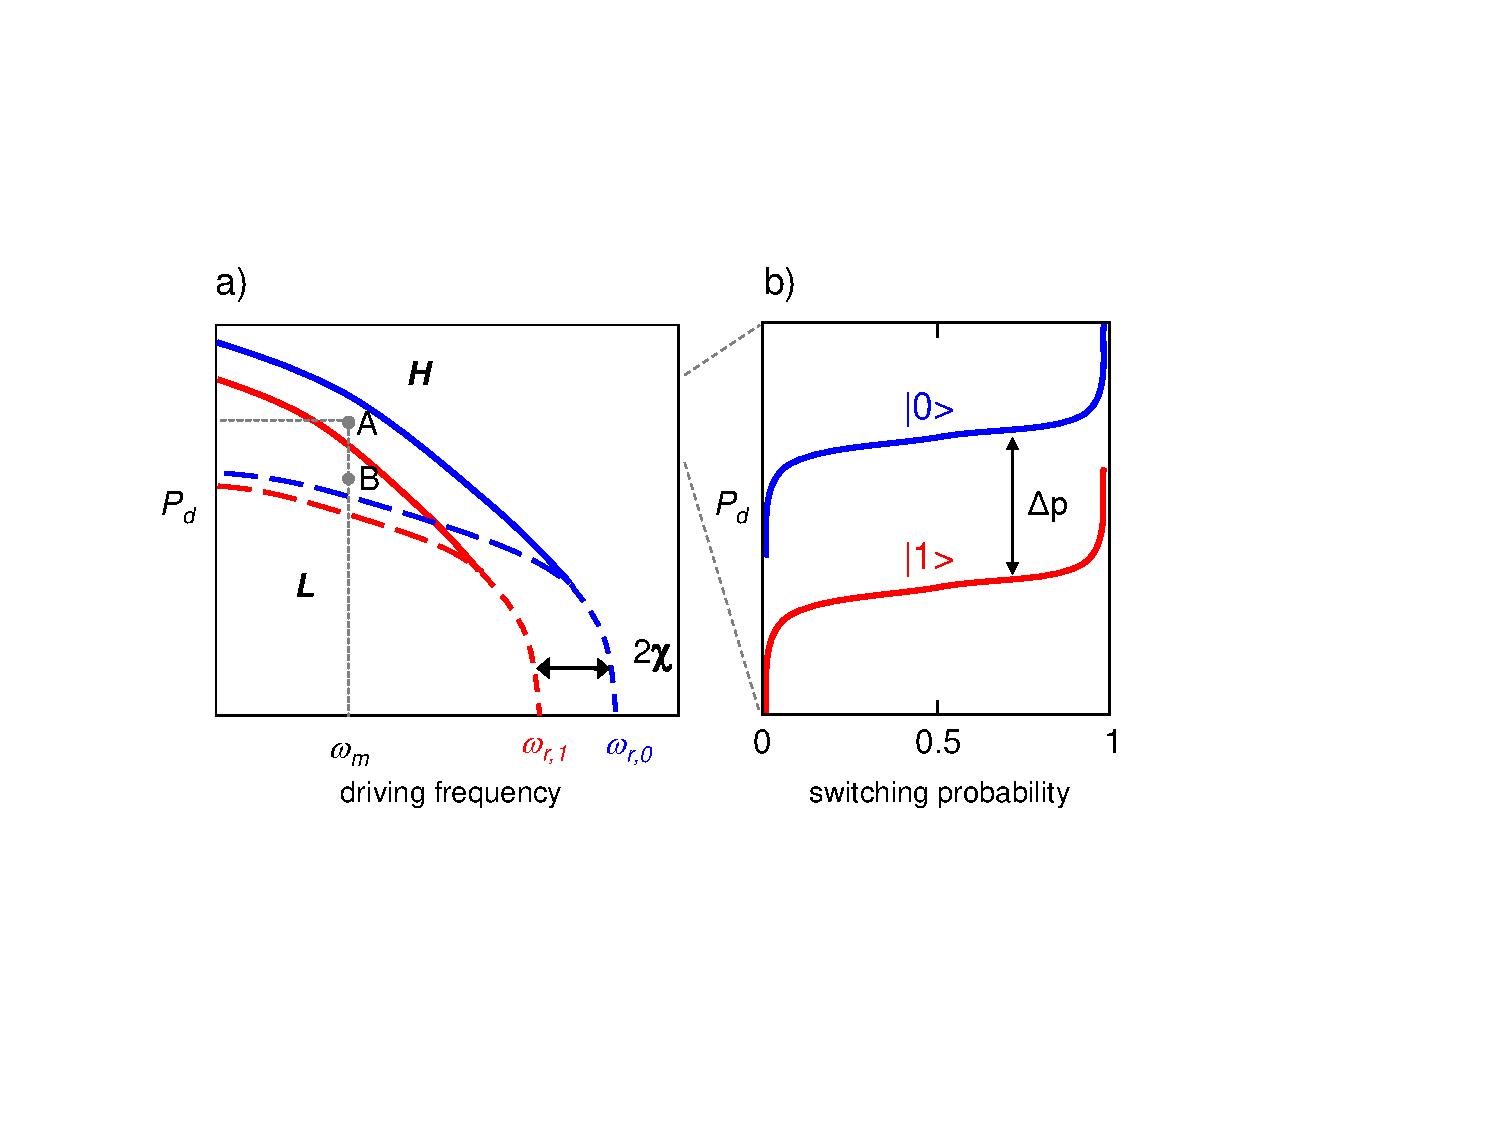
\includegraphics[width=0.7\textwidth]{./material/figures/2-qubit-processor/readout_principle}
	\caption[]{a) The switching probability of the CJBA as a function of the input drive power, shown for the qubit in the states $\ket{0}$ and $\ket{1}$. b) The bifurcation diagram of the CJBA, shown for the qubit in the states $\ket{0}$ and $\ket{1}$. L and H indicate solutions with lows and high amplitude, respectively.}
	\label{fig:readout_process_illustration}
\end{SCfigure}

\begin{itemize}
\item Since the switching of the resonator is a stochastic process, the associated switching probability will exhibit an S-like depedence on the drive power, as shown in fig. \ref{fig:readout_process_illustration}. Now, if the shift of this distribution along the power axis which is induced by the shift of the resonator frequency that depends itself on the state of the qubit is less than the width of the distribution, erronous switching will occur and reduce the fidelity of the readout.
\item If the qubit states changes during the measurement phase, e.g. due to qubit relaxation or excitation, the resonator state will, with high probability, also fall to the state corresponding to the new qubit state, thereby producing a wrong readout signal.
\item If the resonator state changes during the latching phase of the readout, a wrong readout value will occur. This so-called {\it retrapping} can therefore reduce the fidelity of the readout.
\end{itemize}

\subsection{Qubit Decoherence in CQED}

In this section we discuss the relaxation and dephasing mechanisms specific to the CQED architecture.

\paragraph{Relaxation}

In CQED, the qubit is coupled capacitively to a resonator, which itself is coupled to a low-Q input transmission line. The qubit can relax into this transmission line through the gate circuit. The spectral density of gate voltage fluctuations seen by the qubit is given by eq. (\ref{eq:qubit_relaxation_svg}). The resulting relaxation rate is hence
%
\begin{equation}
\Gamma_1^{gate} = 16\pi\beta^2 \omega_{01} \frac{\mathrm{Re}\left(Z(\omega_{01})\right)}{R_K}\left|\bra{0}\hat{n}\ket{1}\right|^2, \label{eq:gate_relaxation_rate}
\end{equation}
%
where $R_K = h/e^2$ and $\beta=C_g/C_\Sigma$. If we assume that the Transmon sees only the impedance of the readout resonator through its gate capacitance, as given by eq. (\ref{eq:lcr_lorentzian}), we can insert the impedance of the resonator into eq. (\ref{eq:gate_relaxation_rate}) and obtain the resulting relaxation rate:
%
\begin{eqnarray}
\Gamma_1^{Purcell} & = & 2\pi\frac{\omega_{01}}{Z_0 \omega_r^2}g_{qr}^2 \mathrm{Re}\left[Z(\omega_{01})\right] \notag \\
                & = & \frac{\pi\kappa}{2}\cdot\frac{g_{qr}^2}{\Delta^2+\kappa^2/4} \label{eq:purcell_rate}
\end{eqnarray}
%
As can be seen, the relaxation rate is proportional to $(\Delta^2+\kappa^2/4)^{-1}$ ($\approx\Delta^{-2}$ for $\Delta \gg \kappa$). The relaxation (or emission) rate of the Transmon compared to the relaxation rate of a qubit get thus modified by the presence of the resonator, which is the so-called {\it Purcell effect} \citep{purcell_spontaneous_1946}. For our processor, this effect is advantageous since it shields the qubit from the low impedance environment presented by the input transmission line and increases thus its relaxation time compared to a direct gate coupling to the input line.

\paragraph{Dephasing} Besides the usual dephasing mechanisms due to the presence of gate charge noise and flux noise in the junction loop, dephasing can occur due to photon-number fluctuations in the resonator which affect the qubit frequency through to the capactivite coupling between the qubit and the resonator \citep{bertet_dephasing_2005,bertet_dephasing_2005-1,rigetti_superconducting_2012}.

\smallskip

The sensitivity of the qubit to photon number fluctuations in the dispersive limit can be derived from the Hamiltonian in eq. (\ref{eq:dispersive_interaction}) as
%
\begin{equation}
\delta \hat{H}_{\bar{n}}=\hbar\delta\bar{n}\chi\hat{\sigma}_z = -\frac{\hbar}{2}\left(\hat{D}_{\bar{n}}\cdot\sigma_z\right)\cdot \delta \bar{n}
\end{equation}
%
(ok, I still need to figure out how I do the derivation of the dephasing rate here, maybe more discussion with Patrice required...)
%
\begin{equation}
\int d\tau C(\tau) = \bar{n}(\bar{n}+1)\exp{\left(-\kappa |\tau|\right)}
\end{equation}
%

%
\begin{equation}
\Gamma_\phi = \chi^2\cdot \frac{\bar{n}_{th}\left(\bar{n}_{th}+1\right)}{\kappa}
\end{equation}
%

\subsection{Qubit-Qubit Interaction}

In this section we discuss possible qubit-qubit coupling schemes. We regard a direct coupling scheme involving a capacitive coupling between two qubits and an indirect scheme involving the coupling of multiple qubits to a resonator which acts as a {\it quantum bus}.

\subsubsection{Direct Capacitive Coupling}

A direct capacitive coupling $C_{qq}$ between two qubits yields a coupling Hamiltonian of the form
%
\begin{eqnarray}
\hat{H}_{qq} & = & \frac{1}{2}C_{qq}\hat{V}_{qq}^2 = \frac{1}{2}C_{qq}\left[\frac{2e}{C_{\Sigma 1}}(n_{g1}-\hat{n}_1)-\frac{2e}{C_{\Sigma 2}}(n_{g2}-\hat{n}_2)\right]^2 \\
& = & \frac{4e^2 C_{qq}}{C_{\Sigma 1}C_{\Sigma_2}}\hat{n}_1\hat{n}_2+\hdots \label{eq:cqed_capacitive_coupling}
\end{eqnarray}
%
Again, this equation is valid in the limit where $C_{qq} \ll C_{\Sigma 1},C_{\Sigma 2}$. For larger capacitances $C_{qq}$ the coupling gets renormalized by a factor $\alpha = 1/(1-C_{qq}^2/[C_{\Sigma 1}C_{\Sigma 2}])$ \citep{nguyen_cooper_2008}. Rewriting this coupling in the basis of uncoupled qubit states yields the effective Hamiltonian
%
\begin{equation}
\hat{H}_{qq} = \hbar g_{qq}\left(\sigma^+_1\sigma^-_2+\sigma^-_1\sigma^+_2\right), \label{eq:cqed_qubit_interaction_hamiltonian}
\end{equation}
%
where $\sigma^+=\ket{1}\bra{0}$ and $\sigma^-=\ket{0}\bra{1}$ and $\sigma_1^\pm=\sigma^\pm\otimes \mathrm{I}$, $\sigma_2^\pm = \mathrm{I}\otimes \sigma^\pm$ and where we have defined the effective qubit-qubit coupling as $\hbar g_{qq} = 4e^2 C_{qq}/C_{\Sigma 1}C_{\Sigma 2}$. Full energy exchange between the qubits is achieved when the qubit frequencies are in resonance. For the more general case of two coupled n-level Transmons, the coupling Hamiltonian takes a slightly more complicated form, as discusses in the Appendix of this thesis. The time evolution operator of the Hamiltonian in eq. (\ref{eq:cqed_qubit_interaction_hamiltonian}) yields a swapping interaction of the form
%
\begin{equation}
i\mathrm{SWAP}(t,\Delta) = \left(
			\begin{array}{cccc}
				1 & 0 & 0 & 0 \\
				0 & \cos{t g_{e}}-i\frac{\Delta}{g_e}\sin{t g_{e}} & i \frac{g_{qq}}{g_e}\sin{t g_{e}} & 0 \\
				0 & i\frac{g_{qq}}{g_e}\sin{t g_{e}} & \cos{t g_{e}}+i\frac{\Delta}{g_{e}}\sin{t g_{e}} & 0 \\
				0 & 0 & 0 & 1 \\
			\end{array}
	\right) \label{eq:swap_with_detuning}
\end{equation}
%
where $\Delta = \omega_{01}^2-\omega_{01}^1$ is the detuning between the qubits and $g_e = \sqrt{4g_{qq}^2+\Delta^2}$ is the effective swapping frequency. Using this interaction, it is straightforward to implement e.g. an $\sqrt{i\mathrm{SWAP}}$ or $i\mathrm{SWAP}$ quantum gate by tuning the qubits non-adiabatically from an off-resonant condition $\Delta \gg g_{qq}$ to a resonance-condition $\Delta = 0$ and letting them interact there for a well-defined amount of time before re-establishing the large detuning ($t=\pi/4g_e$ for the $\sqrt{i\mathrm{SWAP}}$ gate and $t=\pi/2g_e$ for the $i\mathrm{SWAP}$ gate).

\subsubsection{Coupling Bus}

For this particular coupling scheme, we consider two (or more) Transmon qubits coupled to the same resonator. Blais {\it et. al.} \citep{blais_quantum-information_2007} showed that extending the single-qubit rotating-wave Hamiltonian as given in eq. (\ref{eq:cqed_rotating_wave}) to this case of two qubits coupled to a resonator yields an effective qubit-qubit coupling Hamiltonian of the form
%
\begin{eqnarray}
\hat{H}_{2q} & = & \hbar\frac{g_1 g_2(\Delta_1+\Delta_2)}{2\Delta_1\Delta_2}(\sigma_1^+\sigma_2^-+\sigma_1^-\sigma_2^+) \label{eq:cqed_bus_coupling}
\end{eqnarray}
%
This approximation is valid in the limit of large qubit-resonator detuning where $\Delta_1 \gg g_1,\Delta_2 \gg g_2$ with $\Delta_{1,2} = \omega_{01}^{1,2}-\omega_r$ the detuning of the $\ket{0}\to\ket{1}$ transition frequency of each qubit to the bus resonator. Full energy-exchange between the qubits is achieved when the qubit frequencies are in resonance. By detuning the qubits from the resonator, the effective coupling constant can be varied, which is advantageous in many settings. The time evolution operator resulting from eq. (\ref{eq:cqed_bus_coupling}) is identical to eq. (\ref{eq:swap_with_detuning}) when taking into account the modified coupling constanct $g_{qq,r}=g_1 g_2(\Delta_1+\Delta_2)/2\Delta_1\Delta_2$.